\documentclass[conference,a4paper]{IEEEtran}

\usepackage[utf8]{inputenc}
\usepackage[T1]{fontenc}
\usepackage[turkish]{babel}
\usepackage{amsmath,amssymb,amsfonts}
\usepackage{graphicx}
\usepackage{textcomp}
\usepackage{xcolor}
\usepackage{booktabs}
\usepackage{url}
\usepackage{cite}
\usepackage{microtype}
\usepackage{balance}

\def\BibTeX{{\rm B\kern-.05em{\sc i\kern-.025em b}\kern-.08em
    T\kern-.1667em\lower.7ex\hbox{E}\kern-.125emX}}

\begin{document}

\title{TRT tabii \.{I}\c{c}erikleri \.{I}\c{c}in Etkile\c{s}im Platformu\\
\large Engagement Platform for TRT tabii Contents}

\author{\IEEEauthorblockN{Yunus Emre Ar\i}
\IEEEauthorblockA{\textit{Bilgisayar M\"{u}hendisli\u{g}i B\"{o}l\"{u}m\"{u}} \\
\textit{Kocaeli \"{U}niversitesi}\\
Kocaeli, T\"{u}rkiye \\
yunuseemreari@gmail.com}
}

\maketitle

\begin{abstract}
Bu \c{c}al\i\c{s}ma, TRT tabii dijital yay\i n platformundaki dizi, film ve program i\c{c}eriklerinin pasif izleme deneyiminden \c{c}\i kar\i larak quiz ve oyunla\c{s}t\i rma yoluyla etkile\c{s}imli hale getirilmesini sa\u{g}layan, kurumsal \"{o}l\c{c}eklenebilirlikte ve API-first bir backend platformunun mimari tasar\i m\i n\i, ger\c{c}eklenmesini ve canl\i\ da\u{g}\i t\i m\i n\i\ sunmaktad\i r. Geleneksel istemci odakl\i\ quiz sistemlerindeki do\u{g}ru cevap s\i z\i nt\i lar\i, s\"{u}re manip\"{u}lasyonlar\i, a\u{g} kesintilerinde \c{c}ift i\c{s}lem riskleri ve y\"{u}ksek trafikte s\i ralama sorgular\i n\i n getirdi\u{g}i darbo\u{g}azlar; sunucu otoriter oyun motoru, transactional outbox/inbox desenli asenkron mesajla\c{s}ma ve generation tabanl\i\ Redis \"{o}nbellek modeliyle \c{c}\"{o}z\"{u}lm\"{u}\c{s}t\"{u}r. \c{C}ekirdek sistem, da\u{g}\i t\i k transaction karma\c{s}as\i ndan ka\c{c}\i nmak amac\i yla Clean Architecture prensipleriyle mod\"{u}ler monolit olarak tasarlanm\i\c{s}; okuma-yo\u{g}un s\i ralama y\"{u}k\"{u} ise ba\u{g}\i ms\i z \"{o}l\c{c}eklenebilen bir Spring Boot mikroservisine ayr\i\c{s}t\i r\i lm\i\c{s}t\i r. Geli\c{s}tirilen sistem Oracle Cloud Infrastructure \"{u}zerinde Caddy ters vekiliyle sekiz izole Docker konteyneri halinde canl\i ya al\i nm\i\c{s}; 130 backend, 47 frontend ve ger\c{c}ek Testcontainers senaryolar\i yla do\u{g}rulanm\i\c{s}t\i r.
\end{abstract}

\begin{IEEEkeywords}
TRT tabii, oyunla\c{s}t\i rma, mod\"{u}ler monolit, sunucu otoriter, transactional outbox, idempotency, Spring Boot, RabbitMQ, Redis, PostgreSQL.
\end{IEEEkeywords}

\begin{abstract}
\textbf{\textit{English Abstract}---This paper presents the architectural design, implementation, and live deployment of an enterprise-grade, API-first backend platform that transforms the passive viewing experience of TRT tabii video streaming content into an interactive engagement through quizzes and gamification. Traditional client-centric quiz applications suffer from answer leakage, client-side timer manipulation, race conditions causing duplicate XP rewards, and severe database bottlenecks during real-time leaderboard aggregations. These challenges are resolved by introducing a server-authoritative gameplay engine, asynchronous event-driven messaging powered by the Transactional Outbox/Inbox pattern, and a generation-based Redis caching model. The core system is structured as a Modular Monolith adhering to Clean Architecture principles to eliminate distributed transaction overheads, while the read-heavy leaderboard projection is decoupled into an independently scalable Spring Boot microservice. The resulting platform has been deployed to Oracle Cloud Infrastructure utilizing an 8-container topology behind a Caddy reverse proxy and verified with 130 backend, 47 frontend, and containerized integration test suites.}
\end{abstract}

\begin{IEEEkeywords}
TRT tabii, gamification, modular monolith, server-authoritative, transactional outbox, idempotency, Spring Boot, RabbitMQ, Redis, PostgreSQL.
\end{IEEEkeywords}

\section{G\.{I}R\.{I}\c{S}}
Dijital yay\i n platformlar\i n\i n yayg\i nla\c{s}mas\i yla birlikte kullan\i c\i lar\i n video i\c{c}eriklerini t\"{u}ketim bi\c{c}imi b\"{u}y\"{u}k \"{o}l\c{c}\"{u}de tek y\"{o}nl\"{u} ve pasif bir izleme deneyimine d\"{o}n\"{u}\c{s}m\"{u}\c{s}t\"{u}r. TRT tabii ekosisteminde yer alan zengin dizi, film, belgesel ve \c{c}ocuk program\i\ kataloglar\i; kullan\i c\i\ ba\u{g}l\i l\i\u{g}\i n\i, i\c{c}erik hat\i rlan\i rl\i\u{g}\i n\i\ ve topluluk etkile\c{s}imini art\i racak modern bir oyunla\c{s}t\i rma katman\i na ihtiya\c{c} duymaktad\i r. Bu \c{c}al\i\c{s}man\i n temel amac\i; TRT tabii izleyicilerine b\"{o}l\"{u}m ve i\c{c}erik bazl\i\ yar\i\c{s}ma deneyimi sunan, g\"{u}venilir, \"{o}l\c{c}eklenebilir ve k\"{o}t\"{u}ye kullan\i ma kar\c{s}\i\ korumal\i\ bir backend altyap\i s\i\ geli\c{s}tirmektir. Projede quiz ve puanlama mekanizmas\i n\i n se\c{c}ilme nedeni; izleyicinin izledi\u{g}i yap\i mla do\u{g}rudan zihinsel ba\u{g} kurmas\i n\i\ sa\u{g}lamak, i\c{c}erik t\"{u}ketimini peki\c{s}tirmek ve adil bir rekabet ortam\i\ olu\c{s}turmakt\i r.

Sistemin hedef kullan\i c\i\ kitlesi; TRT tabii izleyicileri, i\c{c}erik ve soru edit\"{o}rleri, operasyon ve y\"{o}netim ekipleri ile gelecekte sisteme entegre edilecek web, mobil ve Smart TV istemcileridir. \c{C}al\i\c{s}man\i n kapsam\i, tek ve dikey bir MVP ak\i\c{s}\i\ \"{u}zerine kurgulanm\i\c{s}t\i r. Bu ak\i\c{s}; i\c{c}eri\u{g}i yay\i nlama, quiz ba\c{s}latma, cevaplama, tamamlama, XP verme ve s\i ralama ad\i mlar\i ndan olu\c{s}maktad\i r.

\c{C}al\i\c{s}ma kapsam\i nda geli\c{s}tirilen sistemin sundu\u{g}u temel teknik katk\i lar \c{s}u \c{s}ekildedir:
\begin{enumerate}
    \item S\"{u}re ve puanlama yetkisi tamamen sunucu saatine ba\u{g}lanarak istemci taraf\i ndaki manip\"{u}lasyonlar engellenmi\c{s}tir.
    \item Yay\i nlanan quiz s\"{u}r\"{u}mleri de\u{g}i\c{s}mez (immutable) k\i l\i nm\i\c{s} ve ge\c{c}mi\c{s} denemelerin veri b\"{u}t\"{u}nl\"{u}\u{g}\"{u} g\"{u}venceye al\i nm\i\c{s}t\i r.
    \item A\u{g} kesintilerinde olu\c{s}abilecek m\"{u}kerrer tamamlama isteklerine kar\c{s}\i\ veritaban\i\ k\i s\i tlamalar\i\ ve append-only i\c{s}lem defteriyle tekil XP kazan\i m\i\ garanti edilmi\c{s}tir.
    \item \.{I}li\c{s}kisel veritaban\i\ ile mesaj broker\i\ aras\i ndaki dual-write problemi Transactional Outbox ve Inbox desenleriyle \c{c}\"{o}z\"{u}lm\"{u}\c{s}t\"{u}r.
    \item PostgreSQL sistemin tek kal\i c\i\ do\u{g}ru kayna\u{g}\i\ (SSOT) olarak konumland\i r\i l\i rken, Redis kaybedilebilir ve yeniden \"{u}retilebilir bir okuma modeli olarak kullan\i lm\i\c{s}t\i r.
    \item \c{C}ekirdek sistem mod\"{u}ler monolit s\i n\i rlar\i yla korunurken yaln\i z okuma-yo\u{g}un s\i ralama bile\c{s}eni ba\u{g}\i ms\i z bir mikroservise ayr\i\c{s}t\i r\i lm\i\c{s}t\i r.
    \item WCAG 2.2 AA standartlar\i na uyumlu eri\c{s}ilebilir medya ve s\"{u}re s\"{o}zle\c{s}mesi sisteme kazand\i r\i lm\i\c{s}t\i r.
\end{enumerate}

\section{S\.{I}STEM GEREKS\.{I}N\.{I}MLER\.{I} VE TASARIM HEDEFLER\.{I}}

\subsection{Fonksiyonel Gereksinimler}
Platformun fonksiyonel gereksinimleri alt\i\ ana ba\c{s}l\i kta toplanm\i\c{s}t\i r:
\begin{itemize}
    \item \textbf{\.{I}\c{c}erik Katalo\u{g}u:} \.{I}\c{c}erik, sezon ve b\"{o}l\"{u}m hiyerar\c{s}isinin taslak, yay\i nda ve ar\c{s}iv durumlar\i yla y\"{o}netimi.
    \item \textbf{Quiz Yazarl\i k:} Edit\"{o}rlerin soru metni, d\"{o}rt se\c{c}enek, eri\c{s}ilebilirlik a\c{c}\i klamas\i, g\"{o}rsel ve s\"{u}re tan\i mlayarak quiz s\"{u}r\"{u}mleri olu\c{s}turmas\i\ ve yay\i nlamas\i.
    \item \textbf{Oynan\i\c{s} ve Cevaplama:} Yay\i nlanm\i\c{s} s\"{u}r\"{u}m \"{u}zerinden s\"{u}re k\i s\i tl\i\ attempt y\"{o}netimi; do\u{g}ru \c{s}\i kk\i n ancak cevap sonras\i nda g\"{o}sterilmesi.
    \item \textbf{\"{O}d\"{u}l Mekanizmas\i:} Ba\c{s}ar\i l\i\ tamamlama sonras\i nda tekil ve kal\i c\i\ XP tan\i m\i.
    \item \textbf{S\i ralama (Leaderboard):} Global ve i\c{c}erik bazl\i\ deterministik s\i ralama hesaplamas\i.
    \item \textbf{Kullan\i c\i\ ve Kimlik Y\"{o}netimi:} G\"{u}venli oturum, \c{s}ifre s\i f\i rlama ve rol bazl\i\ yetkilendirme.
\end{itemize}

\subsection{Fonksiyonel Olmayan Gereksinimler}
Sistem veri b\"{u}t\"{u}nl\"{u}\u{g}\"{u}, g\"{u}venlik, idempotency, eri\c{s}ilebilirlik, g\"{o}zlemlenebilirlik, hata tolerans\i\ ve test edilebilirlik hedefleri do\u{g}rultusunda tasarlanm\i\c{s}t\i r. Veritaban\i\ d\"{u}zeyinde yabanc\i\ anahtar ve tekillik k\i s\i tlamalar\i\ uygulanm\i\c{s}; oturum g\"{u}venli\u{g}inde HttpOnly, Secure ve SameSite \c{c}erezler ile SPA CSRF korumas\i\ ger\c{c}eklenmi\c{s}tir.

\subsection{Temel Tasar\i m \.{I}lkeleri}
Sistemin mimarisi be\c{s} temel ilke \"{u}zerine kurulmu\c{s}tur:
\begin{enumerate}
    \item \textbf{SSOT ve Ge\c{c}ici Read Model:} PostgreSQL sistemin tek kal\i c\i\ do\u{g}ru kayna\u{g}\i d\i r; Redis ise h\i zl\i\ s\i ralama sunan ve gerekti\u{g}inde PostgreSQL'den saniyeler i\c{c}inde yeniden \"{u}retilebilen bir \"{o}nbellektir.
    \item \textbf{Son Savunma Hatt\i\ Olarak Veritaban\i:} E\c{s}zamanl\i\ yar\i\c{s} durumlar\i nda (race condition) veri b\"{u}t\"{u}nl\"{u}\u{g}\"{u} yaln\i zca uygulama koduyla de\u{g}il, veritaban\i\ k\i s\i tlamalar\i yla (unique constraint, primary key) garanti edilir.
    \item \textbf{Sunucu Otoritesi:} \.{I}stemci do\u{g}ru cevap ve s\"{u}re otoritesi olamaz; t\"{u}m deadline ve skor hesaplamalar\i\ sunucu saatine g\"{o}re belirlenir.
    \item \textbf{At-Least-Once ve Idempotency:} Mesaj kuyruklar\i ndaki a\u{g} tekrarlar\i na kar\c{s}\i\ t\"{u}keticiler Inbox deseniyle idempotent k\i l\i nm\i\c{s}t\i r.
\end{enumerate}

\section{S\.{I}STEM M\.{I}MAR\.{I}S\.{I}}

\subsection{Genel Mimari ve Katmanlar}
Sistem \"{u}\c{c} ana d\"{u}zlemden olu\c{s}maktad\i r (bkz. \c{S}ekil 1):
\begin{enumerate}
    \item \textbf{\.{I}stemci ve Kenar Katman\i:} React 19 ve TypeScript tabanl\i\ kullan\i c\i\ ve y\"{o}netim aray\"{u}zleri Caddy ters vekili arkas\i nda tek bir HTTPS alan ad\i nda (\url{https://hikayeizi.duckdns.org}) sunulur.
    \item \textbf{Uygulama Katman\i:} Clean Architecture prensipleriyle geli\c{s}tirilen Spring Boot \c{c}ekirdek mod\"{u}ler monolit ile ba\u{g}\i ms\i z \c{c}al\i\c{s}an Leaderboard mikroservisi yer al\i r.
    \item \textbf{Veri ve Mesajla\c{s}ma Katman\i:} Monolith PostgreSQL 17, RabbitMQ 4.1 broker, Leaderboard PostgreSQL 17 ve Redis 8.2 bile\c{s}enlerini kapsar.
\end{enumerate}

\begin{figure*}[t]
\centering
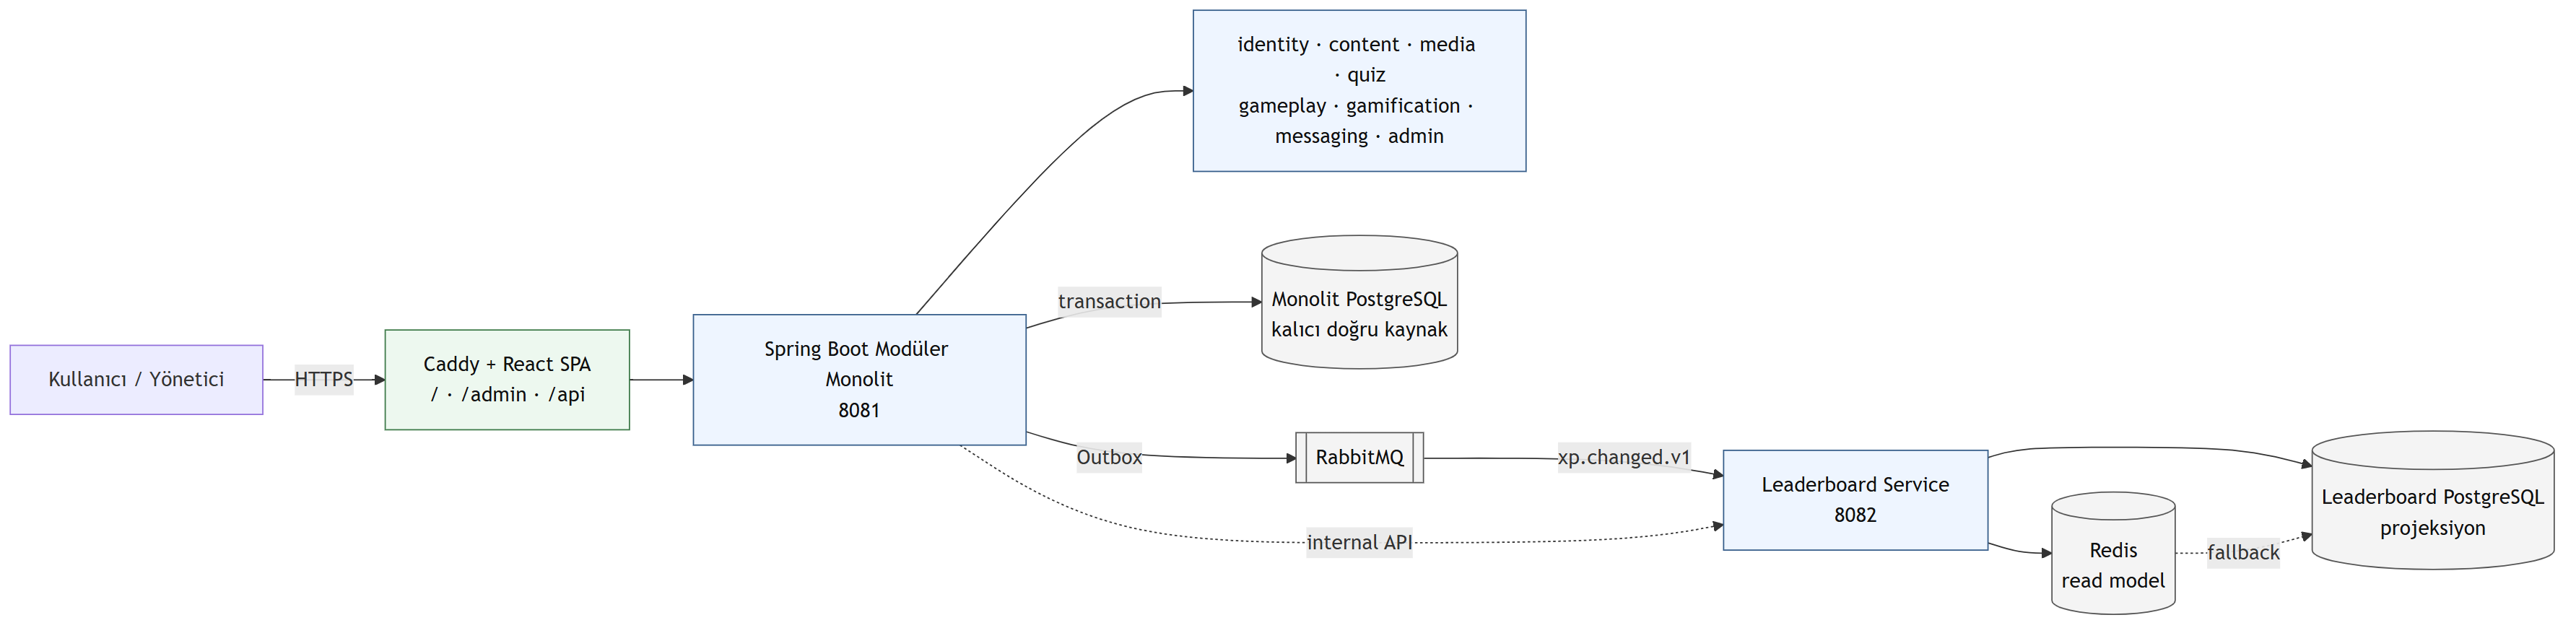
\includegraphics[width=0.88\textwidth]{diagrams/report/01_system_architecture.png}
\caption{TRT tabii i\c{c}erik etkile\c{s}im platformu sistem mimarisi ve mod\"{u}l s\i n\i rlar\i.}
\label{fig:arch}
\end{figure*}

\subsection{Mod\"{u}ler Monolit Yap\i s\i}
\c{C}ekirdek monolit on mant\i ksal mod\"{u}le ayr\i lm\i\c{s}t\i r: \texttt{identity} (hesap ve \c{s}ifre), \texttt{content} (dizi/b\"{o}l\"{u}m katalo\u{g}u), \texttt{media} (g\"{o}rsel depolama ve SHA-256), \texttt{quiz} (soru ve s\"{u}r\"{u}mler), \texttt{gameplay} (attempt ya\c{s}am d\"{o}ng\"{u}s\"{u}), \texttt{gamification} (XP muhasebe defteri), \texttt{messaging} (Outbox/Inbox altyap\i s\i), \texttt{leaderboard} (entegrasyon portu), \texttt{admin} (yetkilendirme) ve \texttt{shared} (ortak modeller). Mod\"{u}ller birbirlerinin tablolar\i na do\u{g}rudan eri\c{s}emez; ileti\c{s}im Java aray\"{u}zleri ve s\"{o}zle\c{s}meler \"{u}zerinden sa\u{g}lan\i r \cite{martin2017clean}.

\subsection{Leaderboard Servisinin Ayr\i\c{s}t\i r\i lmas\i\ (ADR-0031)}
Sistemin tamam\i n\i\ mikroservislere b\"{o}lmek da\u{g}\i t\i k transaction karma\c{s}as\i\ getirece\u{g}inden \c{c}ekirdek domain monolit i\c{c}inde tutulmu\c{s}tur. Yo\u{g}un aggregation ve okuma y\"{u}k\"{u} getiren Leaderboard bile\c{s}eni ayr\i\ bir Spring Boot mikroservisine ta\c{s}\i nm\i\c{s}t\i r \cite{richardson2018microservices}. Monolit d\i\c{s} API'yi sabit tutarken feature flag ile mikroservise y\"{o}nlendirme yapm\i\c{s}, olas\i\ ar\i zalarda yerel fallback mekanizmas\i n\i\ devrede tutmu\c{s}tur.

\section{DOMA\.{I}N VE VER\.{I}TABANI TASARIMI}

\subsection{\.{I}\c{c}erik ve Quiz S\"{u}r\"{u}mleme}
\.{I}\c{c}erik katalo\u{g}u \texttt{content\_catalog\_items}, \texttt{content\_seasons} ve \texttt{content\_episodes} hiyerar\c{s}isinde yap\i land\i r\i lm\i\c{s}t\i r. Quiz yap\i s\i nda tan\i m ile s\"{u}r\"{u}m kavramlar\i\ ayr\i lm\i\c{s}t\i r. Bir quiz s\"{u}r\"{u}m\"{u} yay\i nland\i\u{g}\i\ anda de\u{g}i\c{s}mez (immutable) kabul edilir. D\"{u}zenlemeler otomatik olarak yeni bir s\"{u}r\"{u}m numaras\i yla taslak olu\c{s}turur; bu sayede ge\c{c}mi\c{s} denemelerin b\"{u}t\"{u}nl\"{u}\u{g}\"{u} korunur.

\subsection{Gameplay ve Durum Makinesi}
Kullan\i c\i\ denemeleri kat\i\ bir durum makinesiyle y\"{o}netilir:
\begin{itemize}
    \item \texttt{IN\_PROGRESS}: Deneme ba\c{s}lad\i\u{g}\i nda sunucu saatiyle 30 saniyelik deadline atan\i r.
    \item \texttt{AWAITING\_NEXT\_QUESTION}: Kullan\i c\i\ cevap verdi\u{g}inde saya\c{c} an\i nda dondurulur; sonu\c{c} kart\i nda ge\c{c}irilen s\"{u}re bir sonraki sorudan d\"{u}\c{s}mez.
    \item \texttt{COMPLETED}: T\"{u}m sorular tamamland\i\u{g}\i nda deneme kilitlenir ve sonu\c{c} kesinle\c{s}ir.
\end{itemize}

\subsection{XP \.{I}\c{s}lem Defteri (Append-Only Ledger)}
\texttt{xp\_transactions} tablosu append-only muhasebe defteri mant\i\u{g}\i yla \c{c}al\i\c{s}\i r. Kullan\i c\i\ bir quizi ilk kez tamamlad\i\u{g}\i nda skoruna kar\c{s}\i l\i k gelen XP deftere i\c{s}lenir ve \texttt{gameplay\_quiz\_reward\_claims} tablosuna tekil anahtar at\i l\i r. Tekrar \c{c}\"{o}z\"{u}mlerde kazan\i lan XP s\i f\i r olarak i\c{s}lenir; \"{o}nceki kal\i c\i\ kazan\i m muhafaza edilir.

\begin{figure*}[t]
\centering
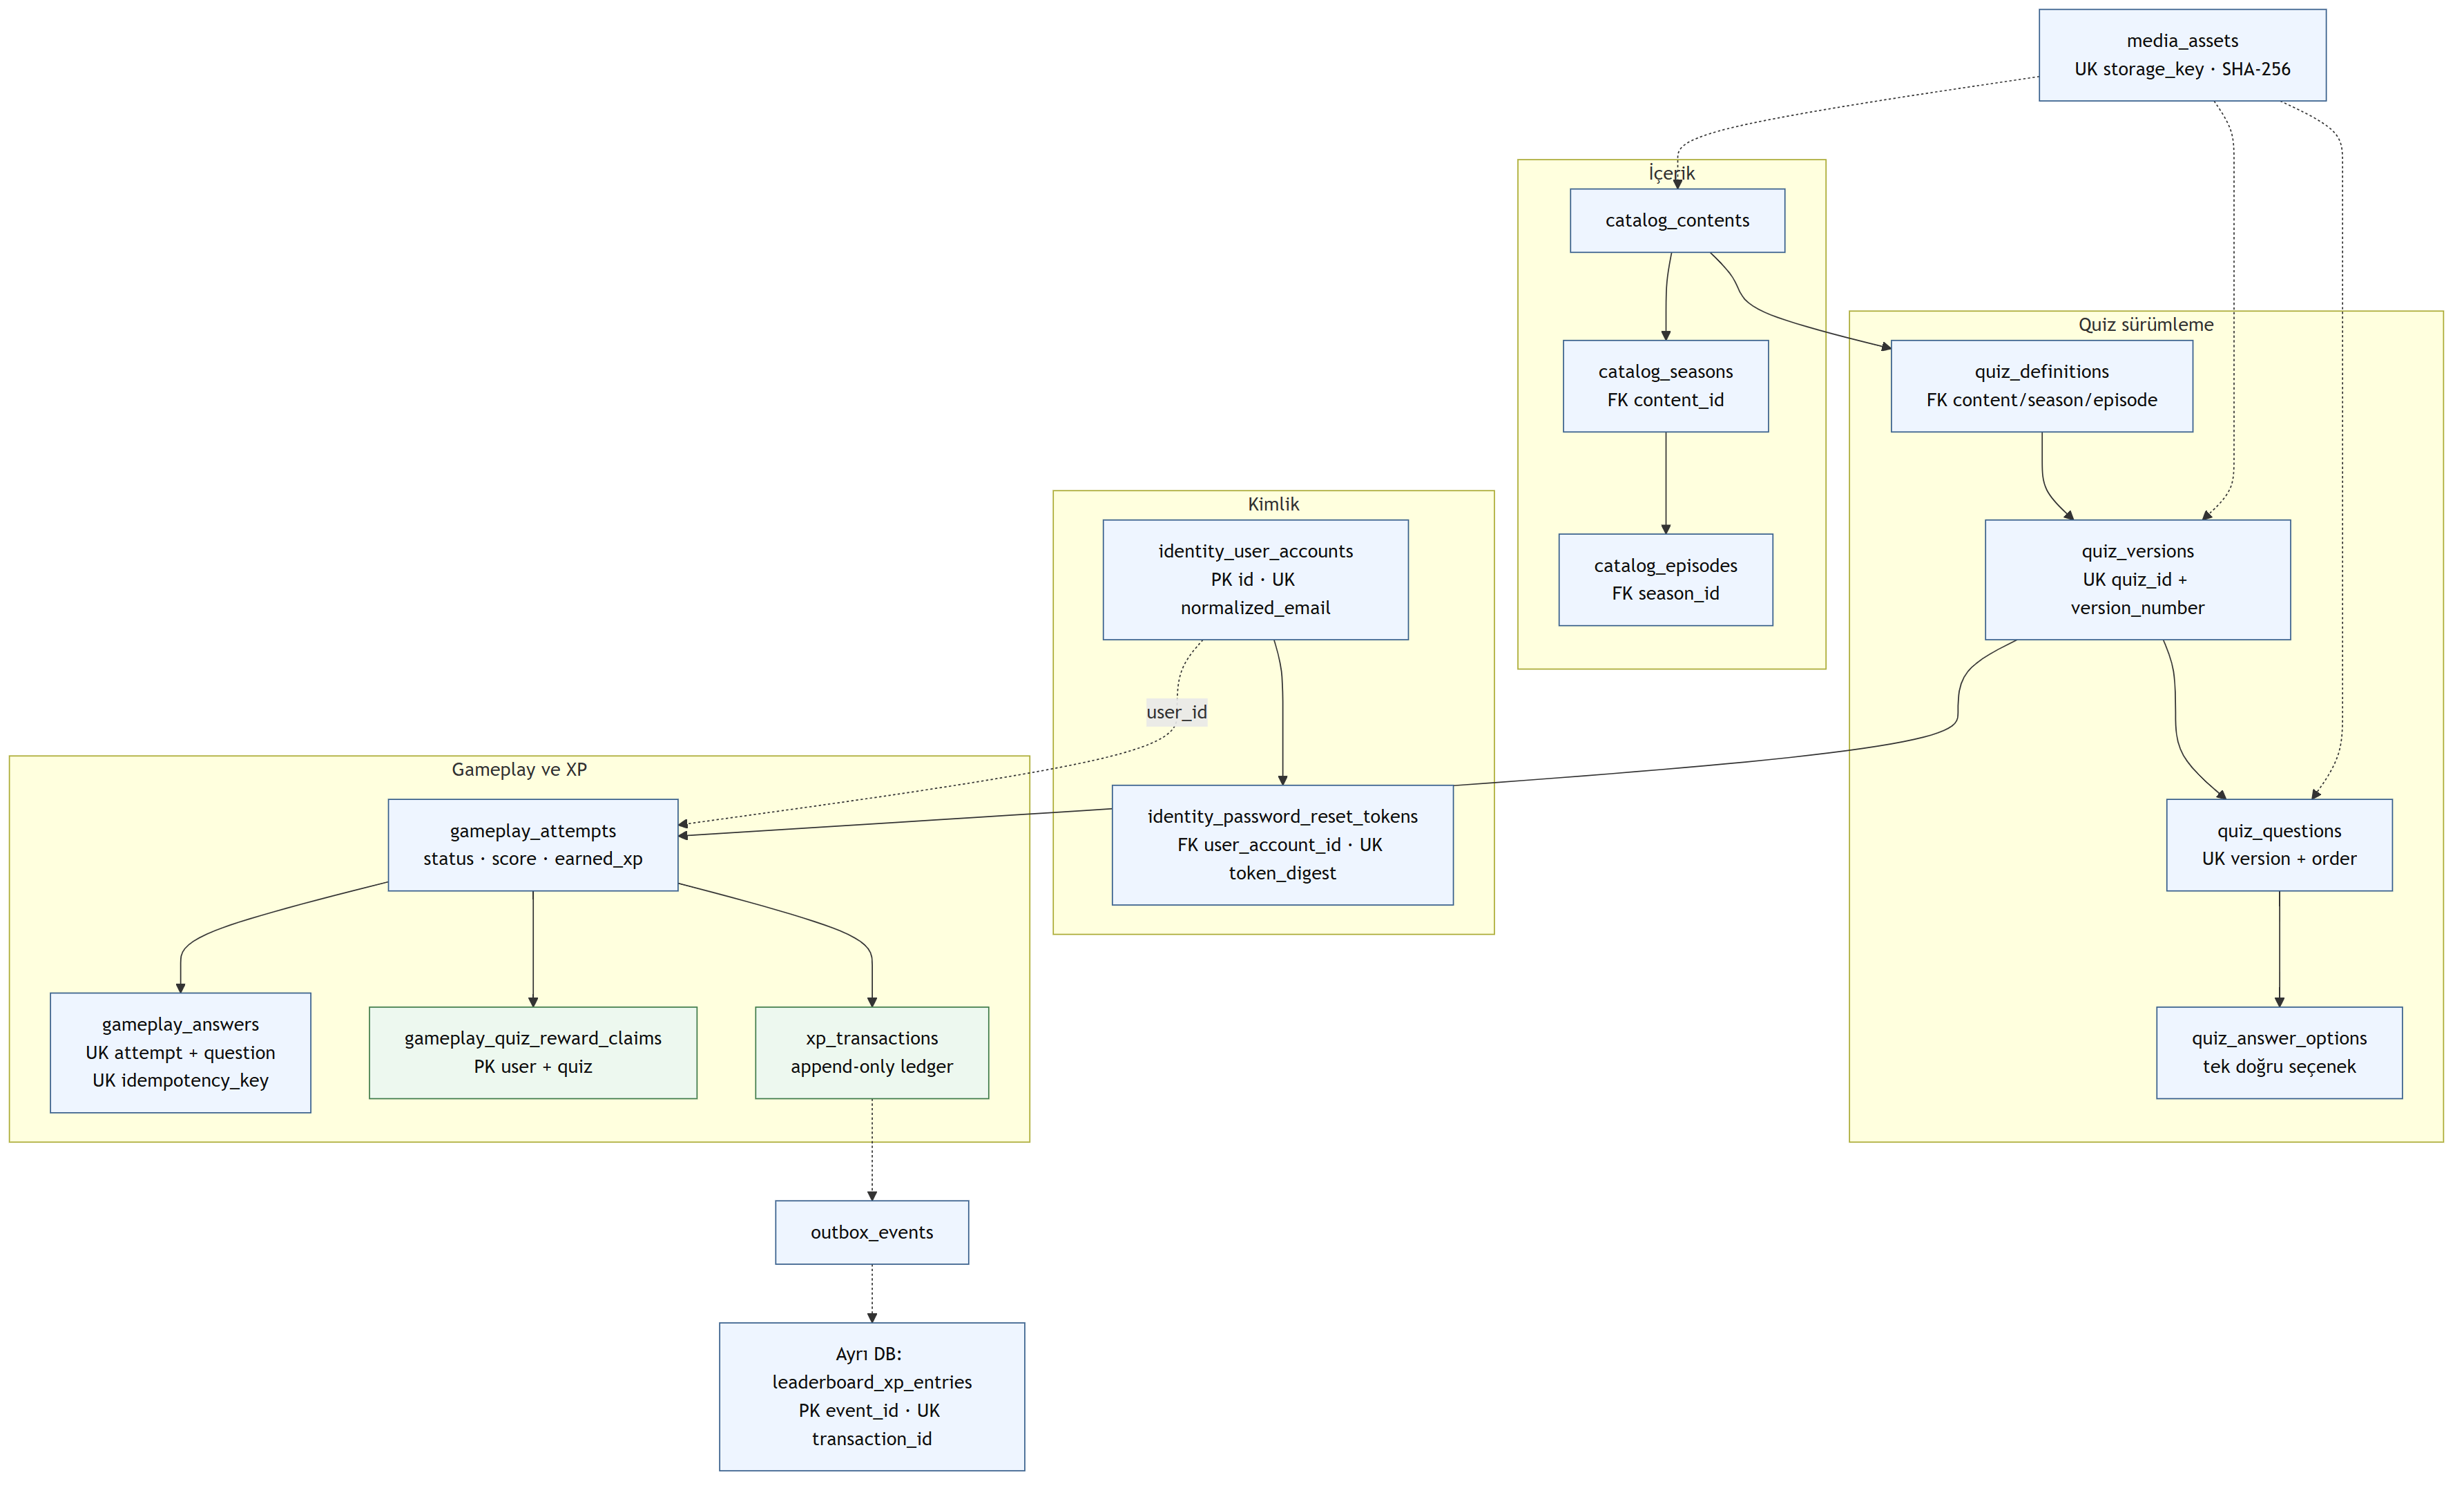
\includegraphics[width=0.88\textwidth]{diagrams/report/02_database_erd.png}
\caption{Monolit \c{c}ekirdek veritaban\i\ ve Leaderboard projeksiyonu varl\i k-ili\c{s}ki modeli (ERD).}
\label{fig:erd}
\end{figure*}

\section{KR\.{I}T\.{I}K S\.{I}STEM AKI\c{S}LARI}

\subsection{Quiz Ba\c{s}latma ve Cevaplama Ak\i\c{s}\i}
Quiz ba\c{s}latma iste\u{g}i geldi\u{g}inde aktif s\"{u}r\"{u}m\"{u}n ilk sorusu \c{c}ekilir, sunucu saatiyle 30 saniyelik deadline hesaplan\i r ve deneme olu\c{s}turulur (\c{S}ekil 3). \.{I}stemciye d\"{o}nen soru modelinde do\u{g}ru \c{s}\i k gizlidir. Kullan\i c\i\ se\c{c}im yapt\i\u{g}\i nda saya\c{c} dondurulur ve sunucuya g\"{o}nderilir. Sunucu s\"{u}reyi do\u{g}rular ($t_{now} \le t_{deadline}$), puan\i\ hesaplar ve cevab\i\ kaydeder. Do\u{g}ru \c{s}\i kk\i n metni ancak bu a\c{s}amada geri bildirim olarak iletilir. Aray\"{u}z sonu\c{c} kart\i ndayken s\i radaki sorunun g\"{o}rselini arka planda \"{o}n y\"{u}kler (preload).

\begin{figure}[htbp]
\centering
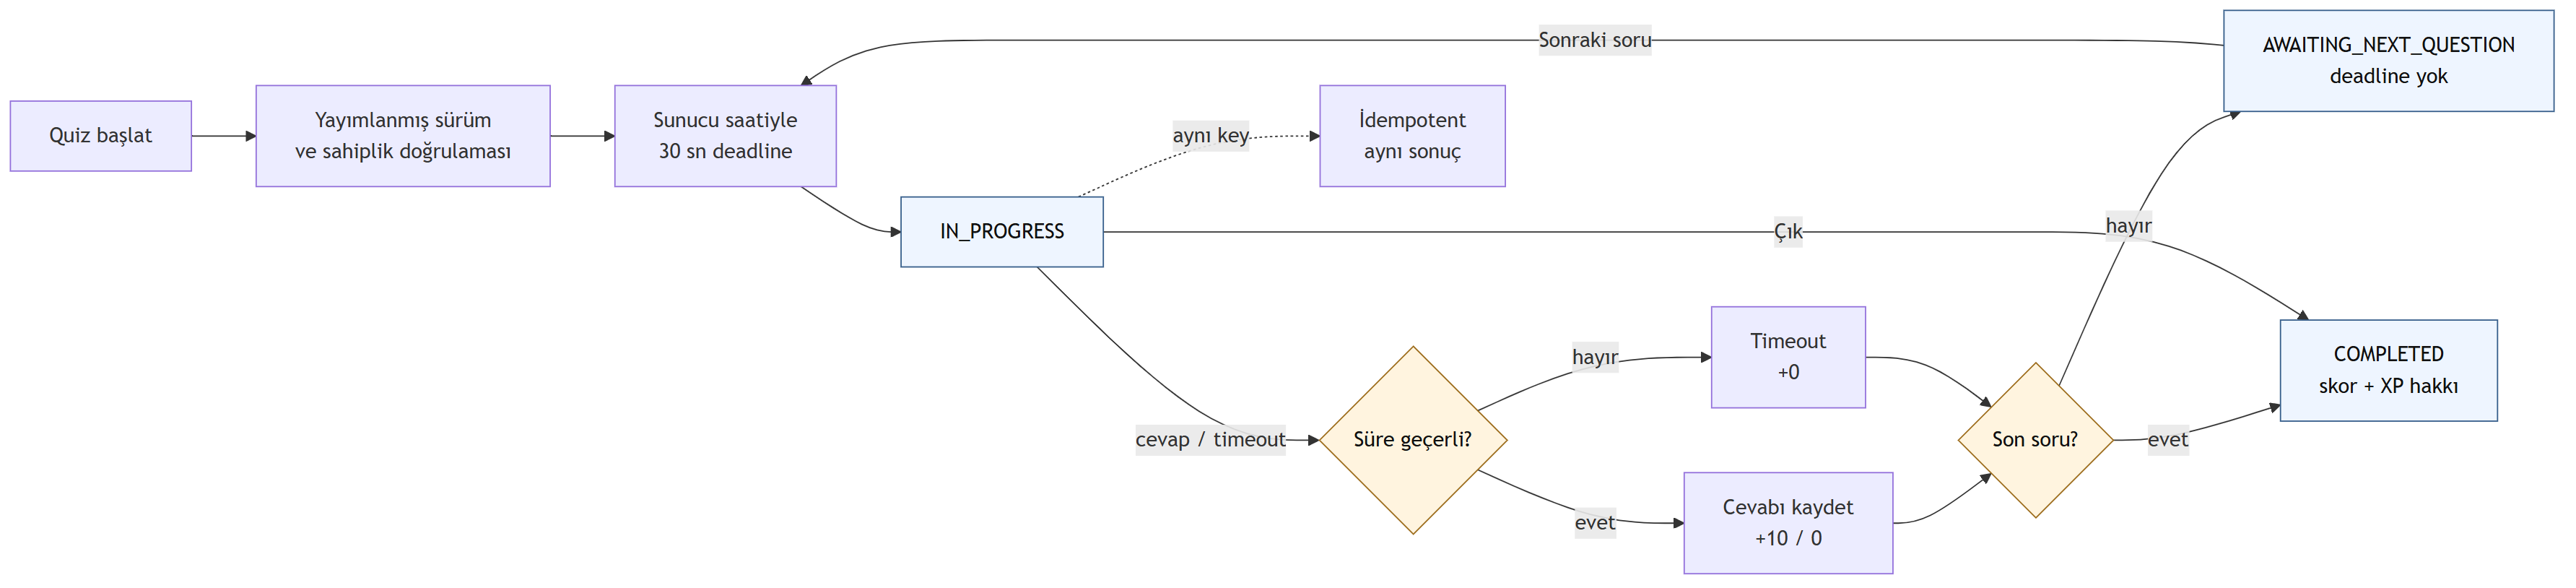
\includegraphics[width=\columnwidth]{diagrams/report/03_gameplay_flow.png}
\caption{Sunucu otoriteli quiz ve gameplay s\i ralama diyagram\i.}
\label{fig:gameplay}
\end{figure}

\subsection{Transactional Outbox ve Inbox Ak\i\c{s}\i}
Quiz tamamland\i\u{g}\i nda attempt durumunun g\"{u}ncellenmesi ile \texttt{outbox\_events} kayd\i\ ayn\i\ yerel PostgreSQL transaction'i i\c{c}inde atomik olarak icra edilir (\c{S}ekil 4). B\"{o}ylece dual-write problemi \"{o}nlenir \cite{richardson2018microservices}. Arka plan yay\i nc\i\ servisi bekleyen olaylar\i\ RabbitMQ'ya iletir (\texttt{publisher confirms} ile). T\"{u}ketici servis mesaj\i\ ald\i\u{g}\i nda \texttt{inbox\_messages} tablosunu kontrol ederek m\"{u}kerrer i\c{s}lemleri engeller.

\begin{figure}[htbp]
\centering
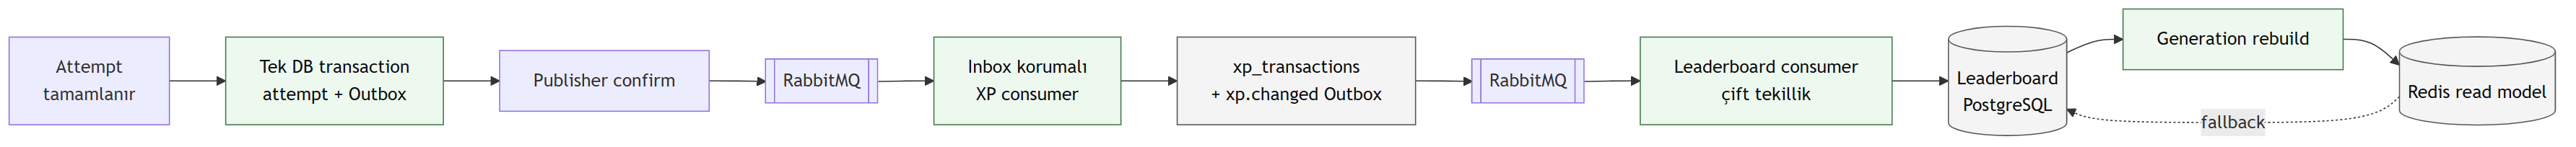
\includegraphics[width=\columnwidth]{diagrams/report/04_outbox_leaderboard_flow.png}
\caption{Transactional Outbox/Inbox ve Leaderboard s\i ralama ak\i\c{s}\i.}
\label{fig:outbox}
\end{figure}

\subsection{Leaderboard ve Generation Tabanl\i\ Redis Modeli}
Leaderboard mikroservisi XP olay\i n\i\ t\"{u}ketir, projeksiyon tablosuna yazar ve toplam XP ile ilk kazan\i m zaman damgas\i n\i\ (tie-break) kullanarak deterministik s\i ralama hesaplar. Redis \'{u}zerinde generation tabanl\i\ anahtarlarla (\texttt{leaderboard:global:\{gen\}}) atomik ge\c{c}i\c{s} yap\i l\i r. Redis devred\i\c{s}\i\ kald\i\u{g}\i nda sistem otomatik olarak PostgreSQL projeksiyonuna geri d\"{u}\c{s}er \cite{redis2025zset}.

\section{G\"{U}VENL\.{I}K, ER\.{I}\c{S}\.{I}LEB\.{I}L\.{I}RL\.{I}K VE DAYANIKLILIK}

\subsection{Kimlik Do\u{g}rulama ve Yetkilendirme}
Parolalar tek y\"{o}nl\"{u} Bcrypt ile tuzlanarak \"{o}zetlenir. XSS riskini engellemek i\c{c}in \texttt{HttpOnly}, \texttt{Secure} ve \texttt{SameSite} nitelikli sunucu oturum \c{c}erezleri kullan\i lm\i\c{s}t\i r \cite{ietf2024cookie}. Durum de\u{g}i\c{s}tiren istekler i\c{c}in SPA CSRF do\u{g}rulamas\i\ zorunlu k\i l\i nm\i\c{s}t\i r. \c{S}ifre s\i f\i rlama token'lar\i n\i n veritaban\i nda yaln\i zca SHA-256 \"{o}zeti saklan\i r (30 dakika ge\c{c}erli, tek kullan\i ml\i k).

\subsection{Quiz G\"{u}venli\u{g}i ve Eri\c{s}ilebilirlik}
Do\u{g}ru cevap istemciye soru \"{o}ncesinde asla iletilmez. G\"{o}rme engelli kullan\i c\i lar i\c{c}in sunulan eri\c{s}ilebilirlik a\c{c}\i klamalar\i\ do\u{g}ru \c{s}\i kk\i\ if\c{s}a etmeden ba\u{g}lam\i\ aktar\i r \cite{w3c2023wcag}. Kullan\i c\i\ tercihi olarak ek s\"{u}re se\c{c}ene\u{g}i tan\i mlanabilmektedir.

\subsection{Kesinti Senaryolar\i}
RabbitMQ kesintisinde attempt tamamlama veritaban\i nda s\"{u}rer, olaylar Outbox'ta birikir. Redis kesintisinde s\i ralama PostgreSQL projeksiyonuna y\"{o}nelir. Leaderboard servisi kapand\i\u{g}\i nda ise \c{c}ekirdek gameplay ak\i\c{s}\i\ kesintisiz i\c{s}lemeye devam eder.

\section{UYGULAMA VE CANLI DA\u{G}ITIM}

\subsection{Kullan\i lan Teknolojiler}
Platform Java 21, Spring Boot 4.1, PostgreSQL 17, Flyway, RabbitMQ 4.1, Redis 8.2, React 19, TypeScript ve Caddy 2 ile ger\c{c}eklenmi\c{s}tir \cite{spring2026boot, postgresql2025doc}.

\subsection{Canl\i\ Da\u{g}\i t\i m Topolojisi (Oracle Cloud)}
Sistem Oracle Cloud Always Free VM (Ubuntu Linux, 12 GB RAM) \"{u}zerinde sekiz Docker konteyneri halinde canl\i ya al\i nm\i\c{s}t\i r. D\i\c{s} d\"{u}nyaya yaln\i zca Port 80 ve Port 443 a\c{c}\i kt\i r; veritabanlar\i\ ve broker izole dahili a\u{g}da (\texttt{app-network}) \c{c}al\i\c{s}\i r. Caddy otomatik TLS (Let's Encrypt) y\"{o}netimi sa\u{g}lar.

\section{TEST VE DO\u{G}RULAMA}

\subsection{Test Stratejisi}
Test piramidi ilkelerine uygun olarak saf domain birim testleri, Testcontainers ile ger\c{c}ek veritaban\i\ ve broker entegrasyon testleri, ArchUnit ile mod\"{u}l s\i n\i r\i\ testleri yaz\i lm\i\c{s}t\i r.

\subsection{\.{I}\c{s} Kural\i\ ve Test Kan\i t\i\ E\c{s}le\c{s}tirmesi}

\begin{table}[htbp]
\caption{\.{I}\c{s} Kural\i\ ve Test Kan\i t\i\ E\c{s}le\c{s}tirmesi}
\label{tab:tests}
\centering
\small
\begin{tabular}{p{2.3cm}p{2.7cm}p{2.6cm}}
\toprule
\textbf{Korunan Risk} & \textbf{Uygulanan Mekanizma} & \textbf{Do\u{g}rulayan Test} \\
\midrule
\c{C}ift cevap verme & Unique k\i s\i t\i\ \& domain kontrol & GameplayIntegrationTest \\
M\"{u}kerrer XP & Reward claim \& defter tekilli\u{g}i & GamificationIdempotencyTest \\
Cevap s\i zmas\i & DTO'dan \c{s}\i kk\i n \c{c}\i kar\i lmas\i & QuizAuthoringIntegrationTest \\
S\"{u}re kayb\i & Awaiting next question durumu & GameplayIntegrationTest \\
RabbitMQ tekrar\i & Inbox tablosu event ID tekilli\u{g}i & MessagingIntegrationTest \\
Leaderboard tekrar\i & Tx ID tekil k\i s\i tlamas\i & LeaderboardServiceIntegrationTest \\
CSRF sald\i r\i s\i & Double submit cookie/header & CsrfProtectionIntegrationTest \\
Admin tekli\u{g}i & Bootstrap tekil kontrol & InitialAdminBootstrapIntegrationTest \\
Token g\"{u}venli\u{g}i & SHA-256 \& tek kullan\i m & AccountAuthenticationIntegrationTest \\
\bottomrule
\end{tabular}
\end{table}

\subsection{Do\u{g}rulama Sonu\c{c}lar\i}
Monolit paketinde 130, Leaderboard servisinde 4 test; frontend paketinde 11 dosyada 47 Vitest testi ve strict TypeScript derlemesi ba\c{s}ar\i yla do\u{g}rulanm\i\c{s}t\i r.

\section{KAR\c{S}ILA\c{S}ILAN SORUNLAR VE M\"{U}HEND\.{I}SL\.{I}K \c{C}\"{O}Z\"{U}MLER\.{I}}

\subsection{PostgreSQL ve RabbitMQ Dual-Write Problemi}
Attempt tamamland\i\u{g}\i nda a\u{g} kesintisi ya\c{s}anmas\i\ durumunda XP olay\i n\i n kaybolmas\i\ riski Transactional Outbox deseniyle \c{c}\"{o}z\"{u}lm\"{u}\c{s}t\"{u}r. Attempt durumu ile olay ayn\i\ yerel transaction'da kaydedilmi\c{s}tir.

\subsection{AWAITING\_NEXT\_QUESTION ve S\"{u}tun Uzunlu\u{g}u S\i n\i r\i}
S\"{u}reyi dondurmak i\c{c}in eklenen durum ad\i\ \texttt{VARCHAR(20)} s\i n\i r\i na tak\i lm\i\c{s}t\i r. Domain dilinin a\c{c}\i kl\i\u{g}\i n\i\ korumak ad\i na durum ad\i\ k\i salt\i lmam\i\c{s}, V18 migration dosyas\i yla s\"{u}tun \texttt{VARCHAR(30)} yap\i lm\i\c{s}t\i r.

\subsection{Sonu\c{c} Ekran\i nda S\i radaki Soru S\"{u}resinin Erimesi}
Kullan\i c\i n\i n sonu\c{c} kart\i n\i\ incelerken ge\c{c}irdi\u{g}i s\"{u}renin sonraki sorudan d\"{u}\c{s}mesi sorunu, cevap an\i nda aktif deadline'\i n silinmesi ve sonraki soru butonuna bas\i ld\i\u{g}\i nda sunucu saatiyle s\i f\i rdan 30 saniye \"{u}retilmesiyle \c{c}\"{o}z\"{u}lm\"{u}\c{s}t\"{u}r.

\subsection{Tekrar \c{C}\"{o}z\"{u}mde XP'nin S\i f\i r G\"{o}r\"{u}nmesi}
Kullan\i c\i n\i n ikinci \c{c}\"{o}z\"{u}m\"{u}nde ana sayfada sıfır XP g\"{o}rmesi sorunu, aray\"{u}z sorgusunun son deneme yerine kullan\i c\i n\i n kal\i c\i\ en y\"{u}ksek tamamlanm\i\c{s} XP de\u{g}erini getirecek \c{s}ekilde g\"{u}ncellenmesiyle d\"{u}zeltilmi\c{s}tir.

\subsection{Canl\i\ A\u{g}da Soru G\"{o}rselinin Gecikmeli Y\"{u}klenmesi}
Canl\i da soru metninin gelip g\"{o}rselin ge\c{c} y\"{u}klenmesi, medya u\c{c} noktas\i na de\u{g}i\c{s}mez (immutable) \"{o}nbellek ba\c{s}l\i klar\i\ verilmesi ve sonu\c{c} kart\i\ a\c{s}amas\i nda s\i radaki g\"{o}rselin arka planda \"{o}nceden indirilmesiyle (preloading) a\c{s}\i lm\i\c{s}t\i r.

\section{TARTI\c{S}MA VE TRADE-OFF DE\u{G}ERLEND\.{I}RMES\.{I}}
\begin{itemize}
    \item \textbf{Mod\"{u}ler Monolit vs Mikroservis:} Geli\c{s}tirme h\i z\i\ ve transaction kolayl\i\u{g}\i\ sa\u{g}lam\i\c{s}; ba\u{g}\i ms\i z da\u{g}\i t\i m esnekli\u{g}i s\i n\i rland\i r\i lm\i\c{s}t\i r.
    \item \textbf{Eventual vs Strong Consistency:} Leaderboard servisinin ayr\i lmas\i\ monolit y\"{u}k\"{u}n\"{u} s\i f\i rlam\i\c{s}; XP ile s\i ralama aras\i nda milisaniyelik bir gecikme kabul edilmi\c{s}tir.
    \item \textbf{Tek Sunucu vs HA:} Oracle Cloud \"{u}zerinde tek sunucu maliyeti s\i f\i rlam\i\c{s}; tek ba\c{s}ar\i s\i zl\i k noktas\i\ (SPOF) bilin\c{c}li bir MVP \"{o}d\"{u}nle\c{s}imi olarak se\c{c}ilmi\c{s}tir.
    \item \textbf{Redis vs \.{I}li\c{s}kisel Sorgu:} Redis s\i ralama sorgular\i n\i\ $O(\log N)$ d\"{u}zeyine indirdi\u{g}i i\c{c}in tercih edilmi\c{s}, senkronizasyon maliyeti \"{u}stlenilmi\c{s}tir.
    \item \textbf{HttpOnly \c{C}erez vs JWT:} \c{C}erez oturumu XSS kar\c{s}\i s\i nda tam g\"{u}venlik ve an\i nda iptal olana\u{g}\i\ vermi\c{s}tir.
\end{itemize}

\section{SONU\c{C} VE GELECEK \c{C}ALI\c{S}MALAR}
TRT tabii i\c{c}erikleri i\c{c}in tasarlanan platform; yay\i nlama, ba\c{s}latma, cevaplama, tamamlama, XP kazan\i m\i\ ve s\i ralama dikey ak\i\c{s}\i n\i\ ba\c{s}ar\i yla tamamlam\i\c{s}t\i r. Gelecekte canl\i\ TV yay\i n ak\i\c{s}\i yla senkronize yar\i\c{s}ma mod\"{u}l\"{u}, WebSocket tabanl\i\ d\"{u}ello altyap\i s\i, merkezi TRT OIDC entegrasyonu ve Kubernetes \"{u}zerinde yatay \"{o}l\c{c}ekleme hedeflenmektedir.

\section*{B\.{I}LG\.{I}LEND\.{I}RME}
Bu \c{c}al\i\c{s}ma, TRT b\"{u}nyesinde ger\c{c}ekle\c{s}tirilen staj program\i\ kapsam\i nda, tabii platformunun etkile\c{s}imli gelece\u{g}ine y\"{o}nelik kurumsal backend mimarilerini ve modern yaz\i l\i m m\"{u}hendisli\u{g}i pratiklerini ara\c{s}t\i rmak ve uygulamak amac\i yla geli\c{s}tirilmi\c{s}tir. S\"{u}re\c{c} boyunca teknik rehberlik sa\u{g}layan TRT m\"{u}hendislik ekiplerine te\c{s}ekk\"{u}r ederiz.

\begin{thebibliography}{10}
\bibitem{spring2026boot} Spring Boot Documentation Team, ``Spring Boot Reference Documentation (v4.1.0),'' VMware Tanzu, 2026.
\bibitem{postgresql2025doc} PostgreSQL Global Development Group, ``PostgreSQL 17.5 Documentation: Concurrency Control and Transaction Isolation,'' 2025.
\bibitem{richardson2018microservices} C. Richardson, \textit{Microservices Patterns: With examples in Java}, Manning Publications, 2018.
\bibitem{rabbitmq2025confirms} RabbitMQ Core Team, ``Reliable Delivery and Publisher Confirms in RabbitMQ,'' Broadcom, 2025.
\bibitem{redis2025zset} Redis Documentation, ``Redis Sorted Sets and Rank Aggregation Mechanics,'' Redis Ltd., 2025.
\bibitem{martin2017clean} R. C. Martin, \textit{Clean Architecture: A Craftsman's Guide to Software Structure and Design}, Prentice Hall, 2017.
\bibitem{w3c2023wcag} World Wide Web Consortium (W3C), ``Web Content Accessibility Guidelines (WCAG) 2.2,'' W3C Recommendation, 2023.
\bibitem{opentelemetry2024w3c} OpenTelemetry Authors, ``W3C Trace Context Specification and Distributed Tracing,'' CNCF, 2024.
\bibitem{evans2003ddd} E. Evans, \textit{Domain-Driven Design: Tackling Complexity in the Heart of Software}, Addison-Wesley, 2003.
\bibitem{ietf2024cookie} Internet Engineering Task Force (IETF), ``HTTP State Management Mechanism (Cookies) and SameSite Attribute,'' RFC 6265bis, 2024.
\end{thebibliography}

\end{document}
